
软件工程和软件架构放在一起会非常复杂,处理不确定性的方法是确保不受潜在风险的影响。我们在人寿保险、健康保险和汽车保险上一直都是这么做的。然而,当涉及到软件开发时,往往会忘记所有的安全预防措施,而只是期望一个乐观的结果。

不仅可能而且会出错,但难以置信的是,测试软件的话题仍然是一个有争议的话题。无论是由于缺乏技能还是缺乏预算,仍然有一些项目缺乏最基本的测试。当客户决定改变需求时,一个简单的修改可能会导致无休止的返工和战争。

当第一次返工发生时,由于没有执行适当的测试而节省的时间就浪费了。如果认为返工不会很快发生,很可能是大错特错的。如今所处的敏捷环境中,返工是日常生活的一部分。我们对世界和客户变更的了解意味着需求的变更,以及对代码的修改。

因此,测试的主要目的是在项目后期节约时间。当需要执行各种测试而不是只关注功能时,这是一项早期投资,但这是一项不会后悔的投资。就像保险政策一样,当事情按照计划进行时,测试需要从预算中拿出一小部分,但当事情变得糟糕时,将获得一笔丰厚的回报。

\subsubsubsection{8.2.1\hspace{0.2cm}测试金字塔}

设计或实现软件系统时,可能会遇到不同类型的测试。每个类的用途略有不同,可以分为以下几类:

\begin{itemize}
\item 
单元测试:代码

\item 
集成测试:设计

\item 
系统测试:需求

\item 
验收测试(端到端或E2E):客户的需求
\end{itemize}

这种区分比较随意,可能经常会看到不同的金字塔,如下所示:

\begin{itemize}
\item 
单元测试

\item 
服务测试

\item 
UI测试(端到端或E2E)
\end{itemize}

这里,单元测试指的是与前面示例相同的层。服务测试是集成测试和系统测试的结合。另一方面,UI测试是指验收测试。

\begin{center}
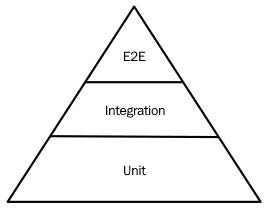
\includegraphics[width=0.6\textwidth]{content/3/chapter8/images/1.jpg}\\
图8.1 -测试金字塔
\end{center}

值得注意的是,单元测试不仅构建成本最低,而且执行速度也非常快,通常可以并行。这就可以创造一个持续集成控制机制。不仅如此,还经常提供关于系统健康状况的最佳反馈。更高级别的测试不仅难以正确编写,而且还可能不够健壮。这可能导致测试结果不稳定,每几次测试运行就有一个会失败。如果高级测试中的失败与单元测试级别上的失败不相关,那么问题很可能是测试本身的问题。

不想说高级测试完全没用,不过应该只专注于编写单元测试,但事实并非如此。看金字塔的形状,因为单元测试应该覆盖基础框架。然而,在此基础上,也应该以适当的比例安排高级测试。不难想象这样一个系统:所有的单元测试都通过了,但系统本身却没有为客户提供价值。一个极端的例子是完美工作的后端,但没有用户界面(无论是图形界面还是以API的形式)。当然,它通过了所有的单元测试,但这都不是无价值的借口!

可以想象,与测试金字塔相反的是冰锥,这是一个反模式。违反测试金字塔通常会导致脆弱的代码和难以跟踪的bug。这使得调试成本的激增,并且在测试开发中也没有节省成本。

\subsubsubsection{8.2.2\hspace{0.2cm}非功能性测试}

已经介绍了所谓的功能测试,目的是检查测试系统是否满足功能需求。但是除了功能性需求之外,还有其他类型的需求是想要控制的。其中一些如下所示:

\begin{itemize}
\item 
性能:应用程序可能会根据功能方面的需求运行,但由于性能较差,最终用户仍然无法使用。我们将在第11章中更多地关注如何提高性能。

\item 
持久性:即使系统确实性能很好,但这并不意味着可以承受持续的高工作负载。当这样做时,它能经受住一些部件的故障吗?当接受了每个软件都是脆弱的,并且可能在任何时刻发生故障的想法时,就要开始设计能够抗故障的系统了。这是Erlang生态系统所采用的一个概念,但这个概念本身并不仅限于Erlang。第13章和第15章中,将更多地提到设计容错系统和混沌工程的作用。

\item 
安全性:没有必要重复安全性的重要性吧!但由于没有得到严肃对待,我们将多次提醒,甚至让开发者感到厌烦。每个连接到网络的系统都可能——而且很可能会——被破坏。在开发过程中应尽早执行安全性测试与其他类型的测试相同:可以在问题修复成本过高之前捕获它们。

\item 
可用性:虽然较差的性能可能会让用户不选择您的产品,但较差的可用性甚至可能让用户理都不理您的产品。虽然性能过载可能会导致可用性问题,但也有其他原因导致的可用性问题。

\item 
完整性:客户数据不应该只受到外部攻击者的保护。它也应该是安全的,不会因为软件故障而发生任何更改或损失。防止位衰减、快照和备份是防止完整性丢失的方法。通过将当前版本与以前记录的快照进行比较,可以确定差异是由所采取的操作造成的,还是由错误造成的。

\item 
可用性:即使产品符合上述所有条件,如果有一个笨拙的界面和不直观的交互,用户可能仍然不满意。可用性测试大多是手动执行的。每当UI或系统的工作流发生变化时,执行可用性评估就很重要。
\end{itemize}

\subsubsubsection{8.2.3\hspace{0.2cm}回归测试}

回归测试通常是端到端测试,可以避免在同一地方跌倒两次。当(QA团队或客户)在生产系统中发现一个bug时,仅仅应用一个热修复程序,并将其遗忘是不行的。

这里需要做的事就是编写回归测试,以防止相同的错误再次进入系统。好的回归测试甚至可以防止同类错误进入生产环境中。毕竟,当知道自己做错了什么,就可以想象其他把事情搞砸的方式。然后,可以做的另一件事是进行原因分析。

\subsubsubsection{8.2.4\hspace{0.2cm}原因分析}

原因分析是用来发现问题的来源的过程,而不仅仅是一个形式。最常见的方法是使用丰田公司著名的5个为什么的方法。这种方法包括剥去问题表象的所有表层,找出隐藏在下面的根本原因。在每一层都问“为什么”,直到找到根本原因。

来看一个实际使用该方法的示例。

问题:我们的一些交易没有收到付款:

\begin{enumerate}
\item 
为什么?系统没有向客户发送合适的邮件。

\item 
为什么?邮件发送系统不支持客户姓名中的特殊字符。

\item 
为什么?邮件发送系统测试不正常。

\item 
为什么?由于需要开发新特性,所以没有时间进行适当的测试。

\item 
为什么?对功能的时间估计不正确。
\end{enumerate}

这个例子中,时间估计的问题可能是在生产系统中发现的错误的根本原因,但这也可能是另一层需要剥离的东西。该框架提供了一种启发式的方法,在大多数情况下是有效的,但如果不完全确定所得到的就是根本原因,可以继续剥离额外的层,直到找到造成所有问题的原因为止。

考虑到许多错误都是由完全相同,且通常是可重复的根本原因导致的,找到根本原因很有用,这样就可以保护自己在未来的几个不同级别上避免犯下相同的错误。这是应用于软件测试和解决问题时的深度防御原则。

\subsubsubsection{8.2.5\hspace{0.2cm}改进的基础}

测试代码可以避免意外的错误,但也开启了不同的可能性。当代码使用测试用例覆盖时,不必担心重构。重构是将完成相应工作的代码转换为功能相似代码的过程,只是它有更好的内部组织。这里可能想知道为什么需要更改代码的组织,这可能有几个原因。

首先,代码可能不具有可读性,这意味着每次修改都需要花费太多的时间。其次,修复的bug会导致其他一些特性的行为不正确,因为随着时间的推移,代码收集了太多的变通方法和特殊情况。这两个原因都可以归结为生产力的提高。从长远来看,会使维护成本更低。

但除了提高工作效率,可能还想提高工作表现。这意味着运行时性能(应用程序在生产环境中的行为)或编译时性能(这是另一种形式的生产率提高)。

通过将当前的次优算法替换为更高效的算法,或者通过正在重构的模块更改所使用的数据结构,可以重构运行时性能。

为了提高编译时性能而进行的重构,通常包括将部分代码移动到不同的编译单元、重新组织头文件或减少依赖关系。

无论最终目标是什么,重构通常都是一件有风险的事情。选择了一些基本可以正常工作的内容,但最终可能会得到更好的版本或更差的版本。怎么知道哪个箱子是对的?这里,测试起到了决定性的作用。

如果当前的特性集完全覆盖,并且想要修复最近发现的bug,那么需要做的就是添加一个将在那时失败的测试用例。当整个测试套件开始通过时,意味着重构工作的成功。

最坏的情况是,若不能在指定的时间范围内满足所有测试用例,必须中止重构。如果想提高性能,可以采用类似的过程,但不是单元测试(或端到端测试),而是将重点放在性能测试上。

随着最近帮助重构和代码维护的自动化工具的兴起(如ReSharper C++: \url{https://www.jetbrains.com/resharper-cpp/features/ReSharperC++}),现在甚至可以将一部分代码单独外包给外部软件服务。诸如Renovate等服务(\url{https://renovatebot.com/}), Dependabot(\url{https://dependabot.com})和Greenkeeper (\url{https://greenkeeper.io/})可能很快就会支持C++。拥有可靠的测试覆盖,可以不用担心在依赖更新期间破坏现有的应用程序。

应该考虑让依赖项在安全漏洞方面保持最新,这样的服务可以减轻负担。因此,测试不仅可以防止犯错,还可以减少引入新特性所需的工作量。还可以改进代码库,并保持其稳定和安全!

理解了测试的必要性,可以开始编写自己的测试。先在没有外部依赖的情况下编写测试,目前只关注测试逻辑。暂时对管理测试结果和报告的细节不感兴趣。因此,将选择一个测试框架来处理这项乏味的工作。下一节中,将介绍一些主流的测试框架。















